\documentclass[ansiapaper]{report}
\usepackage[utf8]{inputenc}
\usepackage[english]{babel}
\usepackage[T1]{fontenc}
\usepackage{amsmath}
\usepackage{amsfonts}
\usepackage{amssymb}
\usepackage{makeidx}
\usepackage{graphicx}
\usepackage{float}
\usepackage{lmodern}
\usepackage[dvipsnames]{xcolor}
\usepackage{tikz}
\usetikzlibrary{intersections}
\usepackage{pgfplots}
\usetikzlibrary{calc}
\usepackage[ansiapaper]{geometry}
\geometry{hmargin=2cm,vmargin=2cm}
\usepackage{fancybox}
\usepackage{mathtools}
\usepackage{enumitem}
\usepackage{tcolorbox}
\usepackage{colortbl}
\usepackage{fancybox}
\tcbuselibrary{most}
\usepackage{pifont}
\usepackage[skip = 5pt, font = {footnotesize}, labelfont = sl]{caption}
\usepackage{subcaption}
\usepackage{eso-pic}
\usepackage{nicematrix}
\usepackage{multicol}
\usepackage{booktabs}
\usepackage{svg}
\usepackage{derivative}
\usepackage{wrapfig}
\usepackage{stmaryrd}
\usepackage{yfonts}
\usepackage{array}
\usepackage{csquotes}
\usepackage[style=phys , backend=biber]{biblatex}
\addbibresource{bibliography.bib}
\author{Andrea}
\setlength{\columnsep}{.5cm}
\usepackage[explicit]{titlesec}
\usepackage{lipsum}
\usepackage{indentfirst}
\usepackage{tabularx}
\usepackage{amsmath}
\usepackage{fancyhdr}
\usepackage{etoolbox}
\usepackage[export]{adjustbox}
\usepackage{fourier-orns}
\usepackage{lettrine}
\usepackage{physics}
\usepackage{hyperref}
\usepackage[titletoc]{appendix}
\usepackage{adforn}
\usepackage{cmbright}
\usepackage{wrapfig}
\definecolor{MyRed}{RGB}{197,112,93}
\definecolor{MySand}{RGB}{208,184,168}
\definecolor{MyWhite}{RGB}{248, 237, 227}
 %% Option 'familydefault' only if the base font of the document is to be sans serif
% use Roman numerals for sections
% \renewcommand\familydefault{\rmdefault}
\renewcommand{\thesection}{\Roman{section}}

% use Arabic numerals for subsections
\renewcommand{\thesubsection}{\Alph{subsection}}

% use letters for subsubsections with a parenthesis
\renewcommand{\thesubsubsection}{\alph{subsubsection})}

% put a period and space after numbers
\titlelabel{\thetitle\thickspace}

% % Make section titles centered and bold
\titleformat{\section}[block]
  {\MakeUppercase\normalsize\sffamily\bfseries}
  {\thesection .}{.3em}
  {\color{black}#1}

  \titleformat{\subsection}[block]
  {\centering\small\sffamily\bfseries}
  {\thesubsection .}{.3em}
  {\color{black}#1}

  \titleformat{\subsubsection}[block]
  {\small\sffamily\bfseries}
  {\thesubsubsection }{.3em}
  {\color{black}#1}
% \titleformat*{\subsection}{\bfseries}

\titleclass{\chapter}{straight}
\titleformat{\chapter}[block]
{\color{white}\large\sffamily\bfseries}
{}
{0em}
{\colorbox{MyRed}{\parbox{\dimexpr\linewidth-2\fboxsep\relax}{\centering \space#1}}}
[]
\titlespacing{\chapter}{0pt}{5pt}{5pt}
\titlespacing{\section}{0pt}{*3}{*3}
\titlespacing{\subsection}{0pt}{*1.5}{*1.5}
\titlespacing{\subsubsection}{0pt}{*1.5}{*1.5}


\hypersetup{
    colorlinks=false,
    linkbordercolor = {white},
    menubordercolor = {white},
    citebordercolor = {black},
    urlbordercolor = {black},
}
\captionsetup{singlelinecheck=off, box=colorbox,boxcolor=MyRed!20, labelsep=endash}

\pgfmathdeclarefunction{gauss}{2}{%
  \pgfmathparse{1/(#2*sqrt(2*pi))*exp(-((x-#1)^2)/(2*#2^2))}%
}
\usetikzlibrary{decorations.markings}
% \renewcommand{\headrule}{%
% \vspace{6pt}\hrulefill
% \raisebox{0pt}{\quad\adforn{64} \adforn{8} \adforn{36}\quad}\hrulefill}
% Page style setup
\pagestyle{fancy}
\fancyhf{} % Clear all header and footer fields

% Set the header height
\setlength{\headheight}{1cm}

% Custom header setup
\fancyhead[L]{%
    \begin{tikzpicture}[overlay, remember picture]
        \node[anchor=north west, xscale=1, yscale=1, minimum width=.7\paperwidth, minimum height=\headheight, fill=MyRed, text=white, inner sep=0pt, outer sep=0pt, line width=0pt] at ([yshift=-0.7cm]current page.north west) {\parbox[c][\headheight]{.7\paperwidth}{\sffamily{\hskip2cm \textbf{\leftmark \hfill \small{Master SdM}\hspace{.5cm} }}}};
        \node[anchor=north east, xscale=1, yscale=1, minimum width=.2\paperwidth, minimum height=\headheight, fill=white, text=MyRed, inner sep=0.5pt, outer sep=0pt, line width=0pt] at ([yshift=-0.7cm, xshift=-1cm]current page.north east) {\parbox[c][\headheight]{.3\textwidth}{\centering\sffamily{\textbf{\small{ENS | ENSL}}}}};
        \draw[MyRed, line width=0.3mm]
        ([yshift=-0.7cm, xshift=-1.75cm]current page.north east)
        rectangle ([xshift=-\paperwidth*0.3+.5cm, yshift=-1.65\headheight-0.3mm]current page.north east);
        \node[fill=MyRed, inner sep=0pt, line width=0pt, minimum width=.12\paperwidth, minimum height=\headheight] (github) at ([yshift=-1.2cm, xshift=.1cm]current page.north east)  {
            \begingroup
            \hypersetup{pdfborder={0 0 0}}
            \hspace{-1.5cm}\href{https://github.com/Chatr0uge/Internship_SPC}{
\includegraphics[height=1cm]{./figures/github.png}}
            \endgroup
    };
    \end{tikzpicture}
}

% Remove the default header rule (optional)
\renewcommand{\headrulewidth}{0pt}

\rfoot{Andrea Combette}
\fancyfoot[C]{\thepage}

\newlength{\tabcont}


\setcounter{tocdepth}{4}
\setcounter{secnumdepth}{4}

\begin{document}

% Custom header setup with tabular



\fontsize{9}{10}\selectfont%

\renewcommand{\contentsname}{Contents} % Rename ToC title


\vskip6pt
\begin{center}
  \noindent \sffamily{\textbf{\Large Lectures notes on Advanced Computational Statistical Physics}}
\end{center}
\vskip9pt

\begin{multicols}{3}

  \renewcommand{\baselinestretch}{1.1}\normalsize % Adjust spacing of ToC
  {\footnotesize \sffamily \tableofcontents} % Set font size for ToC



  \renewcommand{\baselinestretch}{1.0}\normalsize

  \fontsize{9}{10}\selectfont
  \chapter{Introduction}
  \section{Statistical Physics Preliminaries}

  In the 19th century, classical mechanics, rooted in Newton’s laws, dominated physics. Pierre-Simon Laplace famously articulated the deterministic worldview: given the initial conditions of a system, its future could be perfectly predicted through precise mathematical equations. This perspective treated the universe like a clockwork machine, where every event followed from the initial state.

  However, as the study of thermodynamics and many-particle systems advanced, the limits of this purely deterministic approach became clear. Statistical physics emerged to address these complexities, particularly through the work of James Clerk Maxwell and Ludwig Boltzmann. Their pioneering contributions, such as Maxwell's velocity distribution in gases and Boltzmann's statistical interpretation of entropy, introduced probabilistic methods to understand the behavior of large ensembles of particles.

  In this new framework, the precise motion of individual particles became less important; instead, statistical averages and distributions described macroscopic properties like temperature and pressure. While Laplace envisioned a universe governed by strict determinism, statistical physics embraced the unpredictability inherent in large systems, marking a profound shift in understanding.

  This shift continued to resonate into the 20th century, influencing the work of physicists like Philip W. Anderson. Anderson famously argued that "more is different," suggesting that the behavior of complex systems cannot be fully understood by analyzing individual components alone. This echoes the insights of 19th-century statistical physics, where collective behavior emerged from many interacting parts, challenging the reductionist views of classical mechanics.

  In summary, while classical mechanics remained essential for describing deterministic systems, the development of statistical physics in the 19th century introduced a probabilistic approach that transformed our understanding of many-body systems and laid the groundwork for modern physics.

  \section{Computational Statistical Physics}

  Computational methods allow us to simulate these complex systems directly, providing detailed insights into their behavior. Using modern computing power, scientists can model the interactions of millions, or even billions, of particles, making it possible to observe emergent phenomena such as phase transitions, critical behavior, and chaotic dynamics. This computational approach helps us overcome the "many-body" problem, where the sheer number of interactions in a system defies exact solutions.

  One reason computational statistical physics is so powerful is that it can handle systems that are analytically intractable. For instance, systems with strong correlations between particles or those far from equilibrium, which are difficult to study using traditional methods, can be simulated using Monte Carlo techniques, molecular dynamics, and other algorithms.

  Additionally, computational approaches enable the study of phenomena at different scales—from the atomic scale, where quantum effects dominate, to macroscopic scales governed by classical statistical physics. This versatility allows for a deeper understanding of both microscopic mechanisms and their macroscopic consequences, bridging the gap between theoretical models and real-world systems.

  In essence, computational statistical physics allows us to explore systems that are too complex for exact solutions, providing a practical and powerful way to study emergent behavior, phase transitions, and non-equilibrium systems. By leveraging the power of computers, it opens up new frontiers for understanding the vast complexity of the physical world, which neither classical mechanics nor early analytical statistical methods could fully address.

  \begin{figure}[H]
    \centering
    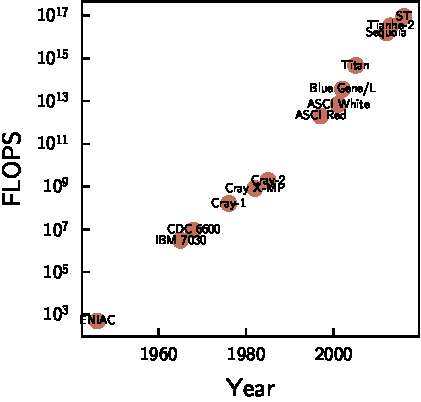
\includegraphics[width=1\linewidth]{./figures/supercomputer_flops.pdf}
    \caption{Number of Floating points operations evolution for the biggest supercomputer \label{fig:supercomputer_flops}}
  \end{figure}

\end{multicols}
\end{document}